\chapter{Experiments on Full Target Dataset}
\label{ch:experiments-full}

The following section covers CBT and LKT-FM ranking experiments performed on the full MovieLens Hetrec 2011 dataset, using Netflix Prize as the source domain. The goal of this experiment is to evaluate the ranking capabilities of CBT on a real dataset without preprocessing.\\
We report an ablation study where additional transformations of the source matrix are applied on baselines, to further analyse whether CBT is capable of knowledge transfer or its performance is strictly bound to the model.\\
Experiments are run over 10 folds for each combination of source and target domains.\\
The kNN phase is performed with cosine similarity to reduce the computational cost of the experiment. The metrics of its results are reported with a cut-off of 20.\\
To compare the results, the following baseline recommender systems are used with the same datasets:
\begin{itemize}
\item \textbf{Random}: random items are chosen for recommendation.
\item \textbf{TopPop}: the most popular items are chosen for recommendation.
\item \textbf{kNN}: the same kNN approach used in CBT is applied, without codebook transfer, on the original target dataset. Only cosine similarity is used and bayesian optimization is applied.
\end{itemize}



\section{Datasets}

\begin{itemize}
\item \textbf{MovieLens Hetrec 2011} \cite{grouplens, hetrec-2011}: 855,598 ratings by 2,113 users on 10,109 movies, with range 1 to 5. The ratings frequency is represented in \autoref{fg:movielens-hetrec-2011-ratings-frequency}
\item \textbf{Netflix Prize} \cite{netflix-prize-dataset}: 100,480,507 ratings by 480,189 users on 17,770 movies, with range 1 to 5. The ratings frequency is represented in \autoref{fg:netflix-prize-ratings-frequency}
\end{itemize}
\begin{table}[hbt]
\centering
\begin{tabulary}{1.0\textwidth}{|L|CCCC|}
\hline
\multicolumn{5}{|c|}{Source Domain} \\
\hline
& Density & Users & Items & Ratings \\
\hline
Netflix Prize & 56.77 & 500 & 500 & 141934 \\
\hline
\hline
\multicolumn{5}{|c|}{Target Domain} \\
\hline
& Density & Users & Items & Ratings \\
\hline
MovieLens Hetrec 2011 & 4.00 & 2113 & 10109 & 855598 \\
\hline
\end{tabulary}
\caption{Properties of the preprocessed datasets used in the experiments on full target dataset.}
\end{table}
\label{tb:full-datasets-properties}
Netflix Prize is preprocessed to extract a very dense dataset to be used as source domain.\\
Preprocessing of the source domain is performed in multiple iterations. First by removing users with a low amount of interactions, then by removing items with a low amount of interactions. Each missing rating of the source domain is filled with the average of ratings of its user.\\
Finally, the preprocessed and full datasets used in the experiments have the properties listed in \autoref{tb:full-datasets-properties}.\\
The target dataset is split in train and test sets. To do so, a random rating for each user is removed from the dataset and added to the test set, while the remaining ratings form the train set.



\section{Ablation Study}

The ablation study for this experiment is performed in three different ways:
\begin{itemize}
\item \textbf{Source domain mix (mixedCBT)}: all the ratings of the source domain are shuffled without keeping rows and column relation, to test whether breaking user and item profile relations has any impact on the performance.
\item \textbf{Random source domain (randomCBT)}: a $500 \times 500$ source domain matrix is randomly generated using uniform distribution with ratings from 1 to 5, to test whether a completely irrelevant source domain leads to worse ranking metrics or the performance of CBT uniquely depends on its model.
\item \textbf{Source domain reduction (removalCBT)}: 10\% of the ratings of the source domain are removed before each missing rating is filled with the average of ratings of its user, to test whether an increase or decrease of source data substantially changes the metrics of the results.
\end{itemize}
Similar source matrix transformations are not applied to LKT-FM due to computational cost.



\section{Hyperparameters}

The hyperparameter values are estimated based on the best results of the previous experiments.\\
The following hyperparameters are set:
\begin{itemize}
\item $\texttt{construct\_validation\_every\_n} = 1$: the amount of iterations after which the codebook construction loss is evaluated by the early stopping training for codebook construction.
\item $\texttt{construct\_lower\_validations\_allowed} = 2000$: the amount of consecutive iterations with loss higher than the best one after which the early stopping training for codebook construction stops.
\item $\texttt{maximum\_construct\_iterations} = 20000$: the maximum amount of iterations used for codebook constructions. If the early stopping training reaches this amount, it stops.
\item $\texttt{transfer\_attempts} = 30$: the amount of attempts to find a local minimum for codebook transfer, as described in \autoref{ss:applied-codebook-transfer}.
\item $\texttt{maximum\_fill\_iterations} = 100$: the maximum amount of iterations used to find a mapping between the target domain and the codebook. The maximum amount is the same for each of the transfer attempts.
\item $\texttt{user\_clusters} = 5$: the amount of user clusters used to build the codebook.
\item $\texttt{item\_clusters} = 5$: the amount of item clusters used to build the codebook.
\item $\texttt{knn\_topk} = 550$: the amount of similar users to consider when computing similarity for kNN.
\item $\texttt{knn\_shrink} = 120$: the shrinkage to apply when computing the similarity for kNN.
\item $\texttt{knn\_similarity} = cosine$: the similarity type to use for kNN.
\item $\texttt{knn\_normalize} = false$: whether to normalize when computing the similarity for kNN. Normalization is computed by dividing the dot product by the product of the norms.
\end{itemize}

\clearpage



\section{Results}

\vspace*{\fill}
\begin{figure}[hbt!]
\centering
\begin{subfigure}{\textwidth}
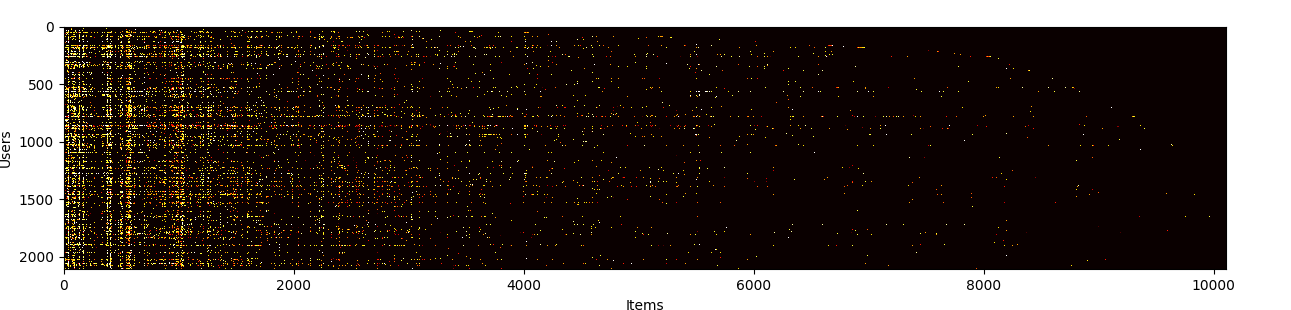
\includegraphics[width=\textwidth]{pictures/movielens-full-target}
\end{subfigure}
\begin{subfigure}{\textwidth}
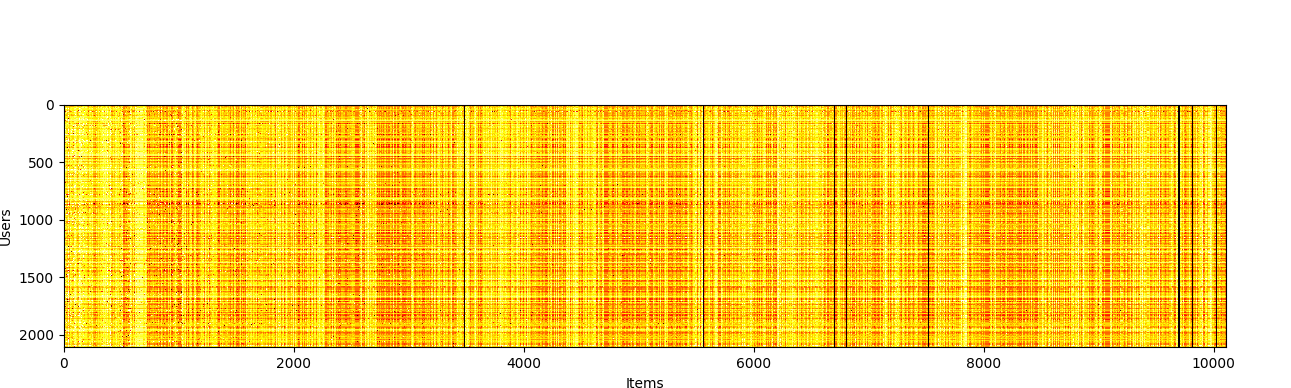
\includegraphics[width=\textwidth]{pictures/movielens-full-target-filled}
\end{subfigure}
\caption{Heatmap of the MovieLens Hetrec 2011 train set before and after the codebook transfer process performed with Netflix Prize as source domain. Low to high values are mapped to red to yellow color scale. Black dots represent missing ratings. The missing ratings in the filled target matrix represent users or items that could not be mapped to clusters during codebook construction, as described in \autoref{ss:codebook-construction}.}
\end{figure}
\vspace*{\fill}

\begin{table}[hbt]
\centering
\begin{tabulary}{\textwidth}{|L|CCC|}
\hline
\multicolumn{4}{|c|}{Netflix Prize $\rightarrow$ MovieLens Hetrec 2011 (Full)} \\
\hline
\hline
Cut-off @20 & mAP & nDCG & Precision \\
\hline
TopPop & 0.0489 $\pm$ 0.0041 & 0.0712 $\pm$ 0.0044 & 0.0076 $\pm$ 0.0003 \\
Random & 0.0004 $\pm$ 0.0003 & 0.0008 $\pm$ 0.0004 & 0.0001 $\pm$ 0.0000 \\
kNN & 0.0672 $\pm$ 0.0027 & 0.0926 $\pm$ 0.0030 & 0.0092 $\pm$ 0.0003 \\
mixedCBT & 0.0103 $\pm$ 0.0012 & 0.0154 $\pm$ 0.0012 & 0.0017 $\pm$ 0.0002 \\
randomCBT & 0.0109 $\pm$ 0.0014 & 0.0161 $\pm$ 0.0015 & 0.0017 $\pm$ 0.0001 \\
removalCBT & 0.0092 $\pm$ 0.0017 & 0.0142 $\pm$ 0.0018 & 0.0016 $\pm$ 0.0002 \\
\hline
CBT & 0.0090 $\pm$ 0.0019 & 0.0134 $\pm$ 0.0022 & 0.0015 $\pm$ 0.0002 \\
LKT-FM & 0.0015 $\pm$ 0.0009 & 0.0024 $\pm$ 0.0012 & 0.0003 $\pm$ 0.0001 \\
\hline
\hline
Cut-off @20 & Recall & Gini Diversity & Item Coverage \\
\hline
TopPop & 0.1513 $\pm$ 0.0068 & 0.0092 $\pm$ 0.0000 & 0.0377 $\pm$ 0.0001 \\
Random & 0.0023 $\pm$ 0.0010 & 0.7222 $\pm$ 0.0001 & 0.9821 $\pm$ 0.0001 \\
kNN & 0.1833 $\pm$ 0.0054 & 0.0489 $\pm$ 0.0004 & 0.2166 $\pm$ 0.0023 \\
mixedCBT & 0.0340 $\pm$ 0.0033 & 0.0087 $\pm$ 0.0003 & 0.0864 $\pm$ 0.0020 \\
randomCBT & 0.0345 $\pm$ 0.0027 & 0.0094 $\pm$ 0.0001 & 0.0915 $\pm$ 0.0012 \\
removalCBT & 0.0324 $\pm$ 0.0035 & 0.0066 $\pm$ 0.0002 & 0.0614 $\pm$ 0.0045 \\
\hline
CBT & 0.0291 $\pm$ 0.0039 & 0.0075 $\pm$ 0.0001 & 0.0807 $\pm$ 0.0029 \\
LKT-FM & 0.0059 $\pm$ 0.0028 & 0.0059 $\pm$ 0.0002 & 0.0612 $\pm$ 0.0044 \\
\hline
\end{tabulary}
\caption{Results of CBT and LKT-FM experiments on full target dataset for cut-off @20 on MovieLens Hetrec 2011 (Full), with Netflix Prize as source domain. The source domain is reduced in order to lower the sparsity. Higher values are better.}
\end{table}

\clearpage



\section{Experiments Summary}

Experiments performed on a real and not preprocessed target dataset confirm the previous conclusions. CBT is heavily outperformed by both simple kNN and TopPop.\\
In addition, CBT provided with a meaningful source matrix is on par with all the three baselines of CBT provided with the transformed and randomly generated source matrices.\\
Nevertheless, it is important to mention that the performance of LKT-FM is very similar to the one of the random recommender system and it is worse than any other baseline. Given the fact that LKT-FM is provided with the same hyperparameters of CBT, including codebook size, and only differs from CBT in implementing alternative models for codebook creation and transfer phases, it is possible to assert that changing the clusters mapping and codebook expansion methods may lead to improved or decreased ranking metrics, compared to the ones obtained with currently known codebook transfer recommender systems. It is also important to mention that, while the results reported by Zang \textit{et al.} in the original LKT-FM article \cite{10.1007/978-3-319-71246-8_39} were not reproducible, the additional hyperparameters for the matrix factorization phase and for the factorization machine were not optimized with bayesian optimization due to the high computational cost.